%% American Dream Stuff

%% if want to use that graph from chetty
\begin{figure}
    \caption{Source: \cite{opportunityinsights}}
    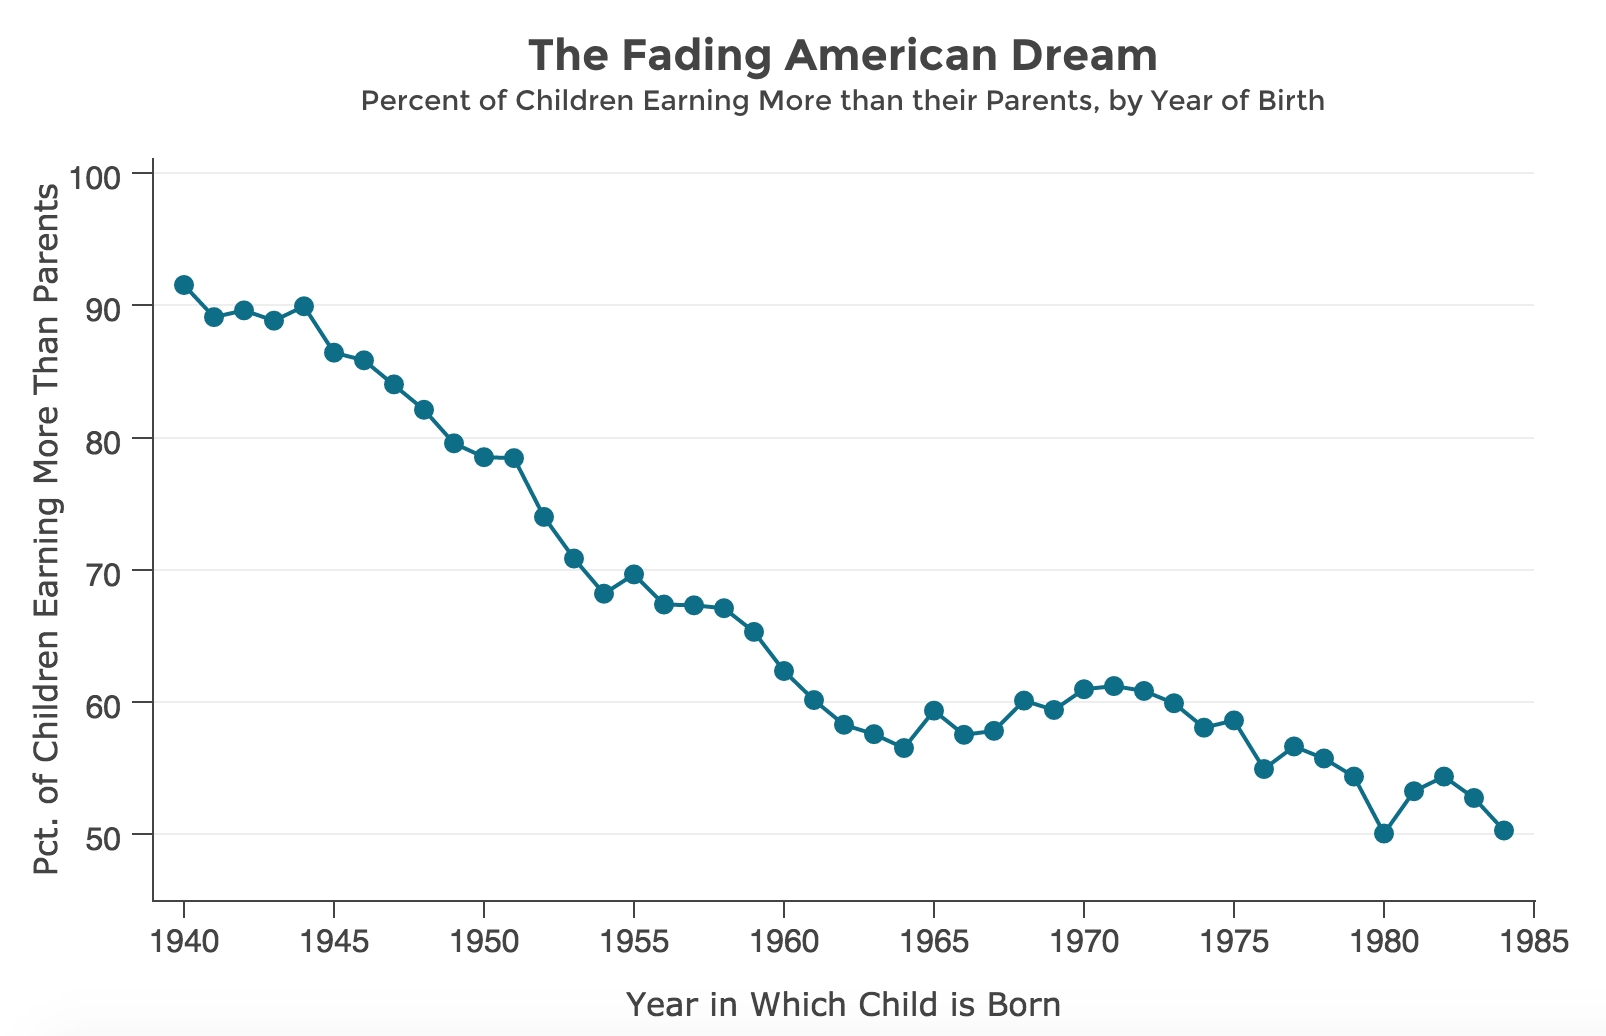
\includegraphics[width=17cm]{chetty_economic_mobility.png}
    \label{fig1}
\end{figure}





%%%%%%%%%%%%%%%%%% rest of overview

Opportunity Insights is a non-profit and partisan organization operating out of Harvard University in Massachusetts. They focus on research using large datasets to locate economic inequity. 
The team has experts in a variety of fields, using the collective disciplines to formulate solutions in battling inequality and poverty \parencite{opportunityinsights}. 
Opportunity Insights is led by Director Dr. Raj Chetty, Professor of Economics at Harvard. 
As part of a broader research initiative to examine the impacts `of  tax  expenditures  on  the  budget  deficit  and  economic  activity', Chetty and his colleagues published the 2014 paper `Where is the Land of Opportunity? The Geography of Intergenerational Mobility in the United States', inspecting economic mobility of the fifty largest cities in the United States, and exploring the classic idea of the `American Dream' \parencite{opportunityinsights, chetty2014}.
Economic Mobility in this case was defined as moving from the bottom fifth income group to the top fifth group. 
They found that mobility was linked with racial and income segregation, income inequality, school quality, access to social capital, and family stability \parencite{chetty2014}.
Areas with high economic mobility were also found to have less segregation and income inequality, while having better schools, stable families, and a larger amount of social capital. (https://opportunityinsights.org/paper/land-of-opportunity/ ). 
Charlotte, North Carolina (NC) was included in this report, and ranked last in terms of economic mobility (Chetty et al., 2014, p. 1). Mecklenburg County was found to be 99 out of 100 counties in terms of economic mobility (https://www.leadingonopportunity.org/about). This shocked those who saw Charlotte as a growing economic hub in the South-East, but not the residents of Charlotte struggling with this economic disparity. 
